% !TeX document-id = {9ccc6fb7-c5f4-4308-9c17-4c226ad62230}
%%%%%%
%
% $Autor: Alpizar, Kumari, JK $
% $Datum: 2023-01-31 11:59:00Z $
% $Version: 1.0.0 $
% $Dateiname: Conclusion
%
% !TeX spellcheck = de_GB
% !TeX program = pdflatex
% !BIB program = biber
% !TeX encoding = utf8
%
%%%


\chapter{Conclusion / Open Questions}

This report explains in detail the method and the tools that are required to digitise the analog meter readings using ESP32 Cam device. Although the model is only trained to recognise and convert 1 digit, this project can be still further developed to recognise all the digits depending on the need. 

Other scope for further developing this project are: 

\begin{enumerate}
	\item Implement a mobile application with user settings and specific account management.
	\item A Log-In module that can track users actions in the application, and responses from the counter.
	\item A more robust HW implementation where the counter detection can be located easily in front of the meter. \ref{fig:Water Meter}
	\begin{figure}  [H]
		\begin{center}
			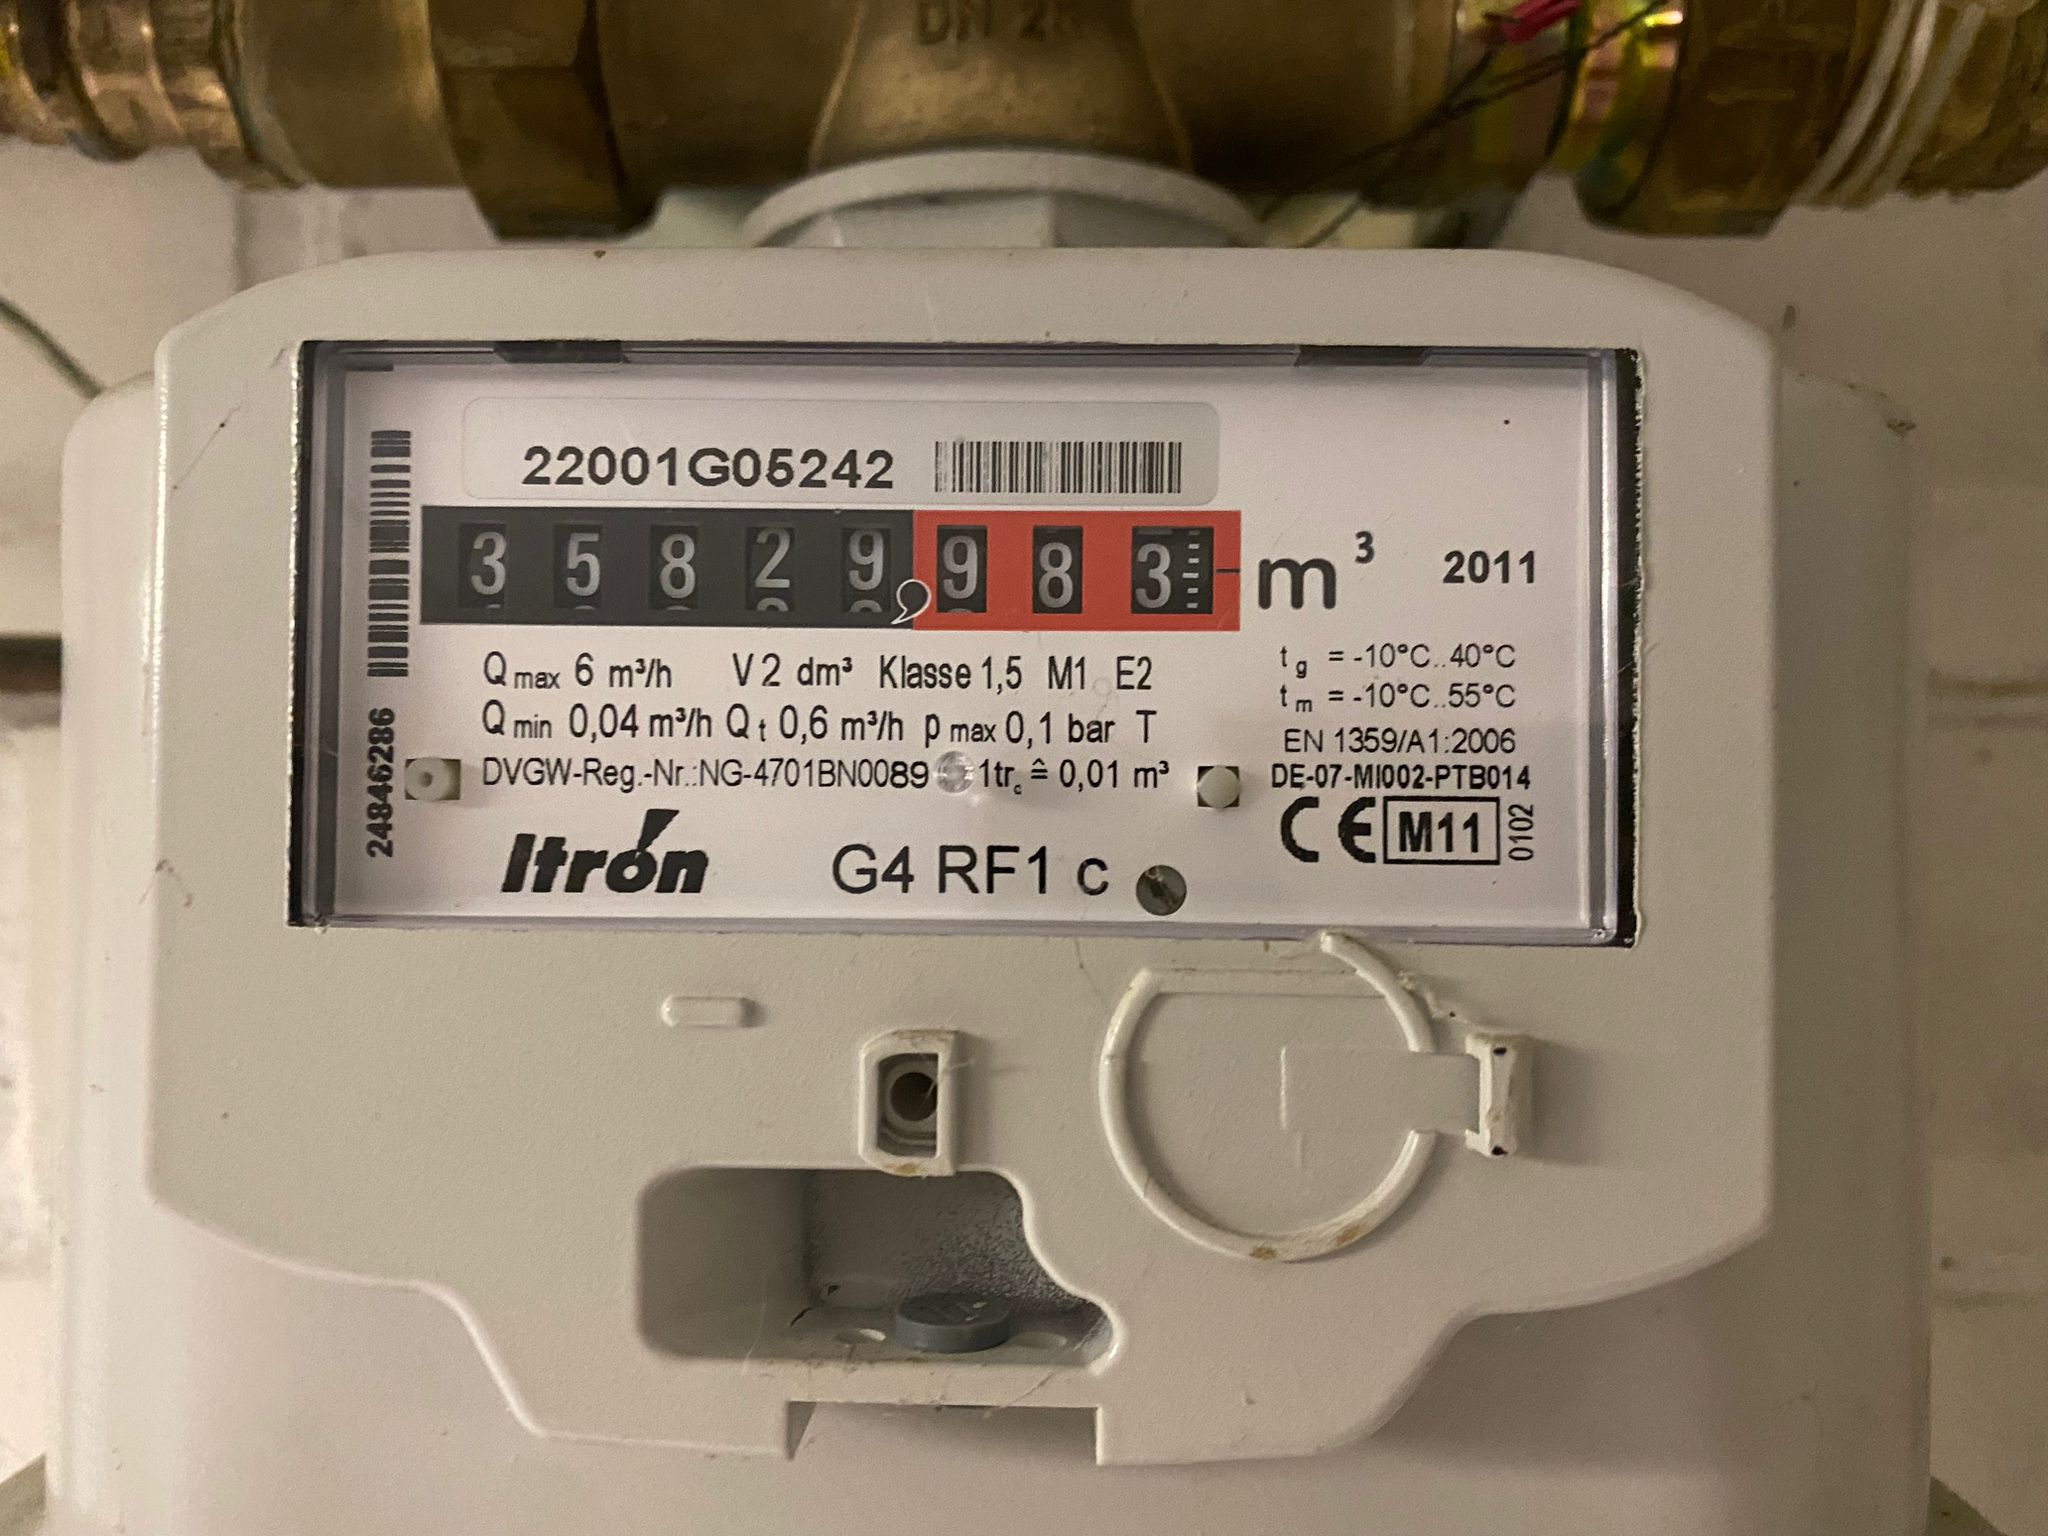
\includegraphics[width=12cm]{ESP32/watermeter}
			\caption{Water Meter} 
			\label{fig:Water Meter}
		\end{center}
	\end{figure}
\end{enumerate}







